% Based on:
% Multics Security Evaluation: Vulnerability analysis
% Paul A. Karger (2nd Lt, USAF)
% Roger R. Schell (Major, USAF)



% # --------------------------------------------------------------------------------- #
\section{Multics Security Evaluation by USAF}

Since on running DPS8-M simulator, you can not really breach security controls. I will describe in short well known evaluation of 
Multics system and how they were able to exploit vulnerabilities in system. 

\textbf{The security evaluation is described in \textit{Multics Security Evaluation: Vulnerability analysis} by P.A. Karger and R.R. Schell} \cite{AnalysisKargerSchell}.

Evaluation of the security of the Multics system had been carried out on the \textit{HIS 645} 
Multics Systems installed at the \textit{Massachusetts Institute of Technology} and at the 
\textit{Rome Air Development Center} in span of March 1972 and June 1973.

The main purpose for this evaluation had been the lack of effective \textit{multi-level security controls}
in US military. The term multi-level (from US Military point of view) means, in the most general case, 
those controls needed to process several levels of \textit{classified material}, from unclassified 
through compartmented top secret in a \textit{multi-processing multi-user computer system with simultaneous 
access} to the system by users with different levels of clearances.

The lack of such effective systems in those days has led the \textit{US Military} to operate computers
in closed environment in which system had been dedicated to the highest level of classified material and
all users had been required to be cleared to \textit{that} level.
Such a systems resulted in extreme insufficient manpower utilization and high costs of deployed systems,
mainly becuase of quantity of dedicated systems. 

Requirements of the \textit{Air Force Data Service Center} (AFDSC) were to be providen with 
\textit{responsive interactive time-shared computer services} to users within the Pentagon
at all \textit{classification levels}. From \textit{unclassified} to \textit{top secret} clearance level.
AFDSC in particular did not wish to incur the expense of \textit{multiple computer systems} nor the expense of 
\textit{encryption devices} for remote terminals which would otherwise be processing unclassified materials.

\textbf{Several more analysis has been done in years after, but this analysis was the key 
for Multics to gain B2 security evaluation mark.}


\subsection{State of "current systems" in early 70's}
% Operating systems does not considered the security as fundamental requirement

The internal controls of current computers repeatedly had been shown \textit{Insecure} through many
\textit{penetration exercises} on system such as \textit{WWMCCS GCOS} and \textit{IBM OS/360/370}.
This insecurity of internal controls had been fundamental weakness of \textit{these} operating systems 
and cannot be corrected by \textit{"patches"}, \textit{"fix-ups"} and \textit{"add-ons"} to these systems.
Rather a \textit{fundamental re-implementation} using an integrated hardware and software design which would 
consider \textbf{security as fundamental requirement}.

It is not sufficient to use a team of experts to \textit{test} the security controls of a system. Such a 
\textit{ZARF "tiger team"} can only show the existence of vulnerabilities but \textit{cannot} 
prove their \textit{non-existence}.

\subsection{Reference Monitor}

The concept of \textit{reference monitor} had been introduced by the \textit{ESD Computer Security 
Technology Panel}. This reference monitor is that hardware and software \textit{combination} which 
must monitor \textbf{all} references by \textbf{any program} to \textbf{any data anywhere} in the 
system to ensure that the security rules are followed, which are defined by:
\begin{itemize}
    \item The monitor must be tamper proof.
    % Tamper = to touch or make changes to something that you should not, 
    % usually without enough knowledge of how it works or when you are trying to damage it
    \item The monitor must be invoked for every reference to data anywhere in the system
    \item The monitor must be small enogh to be \textit{proven correct} 
\end{itemize}

Systems such as GCOS and OS/360 meet just first requirement. The second requirement was generally not met by
systems contemporary in \textit{60s} and \textit{70s}, since they usually include \textit{bypasses} to permit
special software top operate.
The most important, operating systems in those days had been so \textit{large}, so \textit{complex} and 
so \textit{monolithic} that one could not begin to attempt a formal proof or certification of their current 
implementation. 

\subsection{Approach Plan}

An attempt was to be made to operate with same type of ground rules under which a real agent would operate.
That is, with each penetration, and attempt would be made to extract or modify sensitive system data 
without detection by the \textit{system maintenance} or \textit{administrative personnel}.
Several exploitation's had been discovered, such as changing access fields in SDW's, changing protected 
identities in the PDS, inserting trap doors into system libraries and accessing the system password file.

In this paper we are not going to to describe all the vulnerabilities shown by this evaluation, rather just those 
interesting and with the most significant impact on contemporary development of operating systems and its 
security's control systems.

% \subsection{Hardware Vulnerabilities}

\subsection{Subverter routine}

To attempt a gross measure of the rate of security sensitive component failure, a procedure called the 
\textit{subverter} was written to sample the security sensitive hardware on frequent basis, testing for 
component failures which could compromise the security controls.
The subverter was run in the background of an interactive process, once each minute. The subverter was run 
over 1100 hours in a year period on the \textit{MIT 645 System}, during these operating hours no security sensitive 
component failures were detected.
Which points at and gave great result about the concert in a system processing multi-level classified material.
If the hardware is prone to error, potential security vulnerabilities become a significant problem.

\subsection{Instruction Access Check Bypass}

While experimenting with the hardware subverter, a sequence of code was observed which would cause the hardware 
of the 645 to \textit{bypass access checking}. Specifically the \textit{execute} instruction in certain cases 
would permit the executed instruction to access a segment for \textit{reading} or \textit{writing} without the 
corresponding permissions in the SDW.
This vulnerability occurred when the execute instruction was in certain restricted locations of a segment with 
at least \textit{read-execute} permission.
The exact layout of instructions and indirect words was crucial, otherwise the \textit{access checks} were done 
properly.
This bug represents a violation of one of the most fundamental rules of the Multics design concept - the checking 
of \textbf{every} reference to a segment by the hardware.

% \subsection{Software Vulnerabilities}

\subsection{Insufficint Argument Validation}

On the 645 CPU rings mechanism have not been implemented in the way of hardware. (Only after several years on HIS 6180 CPU.) 
Therefore, the protection rings had been implemented by providing \textit{eight descriptor segments} for each user, one 
descriptor segment per ring.
Because the 645 Multics system must simulate \textit{protection rings} in software, there is no direct hardware 
validation of arguments passed in a subroutine call from a \textit{less privileged ring} to \textit{more 
privileged ring}. Some form of validation is required, because a malicious user could call a ring 0 routine 
that stores information through a user supplied pointer.
If the malicious user supplied a pointer to data to which ring 0 had \textit{write} permission but to which the 
user ring did not, ring 0 could be \textit{"tricked"} into causing a security violation.

To provide validation, the 645 \textit{software ring crossing mechanism} requires all gate segments to declare to 
the \textit{"gatekeeper"} the following information:
\begin{enumerate}
    \item number of arguments expected
    \item data type of each arguments
    \item access requirements for each argument - read only or read/write
\end{enumerate} 
This information is stored by convention in specified locations within the \textit{gate segment}. The gatekeeper 
invokes an argument validation routine that inspects the argument list being passed to the gate to ensure that the 
declared requirements are met. If any test fails, the argument validator aborts the call and signals the \textit{"
gate\textunderscore error"} in the calling ring.

In 1973, a vulnerability was identified in the argument validator that would permit the \textit{"fooling"} of ring 0 
programs.
The argument validator's algorithm to validate read or read/write permission was as this:
\begin{enumerate}
    \item Copy the argument list into ring 0 to prevent modification of the argument list by a process 
    running on another CPU in the system while the first process is in ring 0 and has completed argument validation
    \item Force indirection through each argument pointer to obtain the segment number of the target argument
    \item Look up the segment in the calling ring's descriptor segment to check for read or write permission
\end{enumerate}

The vulnerability is as follows:
\begin{itemize}
    \item An argument pointer supplied by the user is constructed to contain an IDC modfier that causes the first 
    reference through the indirect chain to address a valid argument.
    \item The first reference is the one made by the argument validator.
    \item The reference through the IDC modifier increments the address field of the tally word causing it to point 
    to a different ITS pointer which points to an argument which is writable in ring 0 \textbf{only}.
    \item The second reference through this modifier indirect chain is made by the ring 0 program which proceeds 
    to \textbf{write data where it should not}. 
\end{itemize}
%# TODO add 'Figure 5. Insufficient Argument Validation' .pdf (p) 28

This vulnerability resulted from violation of a basic rule of the Multics design, that \textit{all arguments to a more 
privileged ring must be validated}.
The problem was no in the fundamental design, but the lack of \textit{ring hardware} on HIS-645 CPU system.

\subsection{Master Mode Transfer}

The HIS-645 CPU has a \textit{master mode} in which privileged instructions may be executed and in 
which \textit{access checking is inhibited} although address translation through segment and page 
tables is retained. 
The original design of Multics protection rings called for master mode code to be restricted to ring 0 by convention.
This convention caused the \textit{fault handling mechanism} to be excessively expensive due to necessity of switching
from user ring into ring 0 and out again using the full software ring crossing mechanism.

Therefore it was proposed and implemented that the \textit{signaller} module  was permitted to run in the user 
ring to speed up fault processing.

The analysis shows that master mode procedures in the user ring represents a fundamental violation of the Multics 
security concept. Violating this concept moves the security controls from the basic hardware and software mechanism 
to the cleverness of the systems programmer who, \textit{being human, makes mistakes and commits oversights}
The master mode procedures become classical "supervisor calls" with no rules for sufficient security checks.

The master mode \textit{pseudo-operation} code was designed only to protect master mode procedures from random calls 
within ring 0. It was not designed to withstand the attack of a malicious user. By moving the signaller into the user 
ring, the designers allowed a user leaving a core dump and therefore to crash the system.


\subsection{Dump and Patch Utilities}

\textit{This section shows the exploitation by a remote user online}.

To provide support to the system maintenance personnel, the Multics system includes commands to \textit{dump} or 
\textit{patch} any word in the \textbf{entire virtual memory}. These utilities are used to make online repairs while 
the system continues to run. These commands are dangerous, because they \textit{bypass} all security controls to 
access otherwise protected information, and if misused, it can cause crash of the entire system.

To protect the system, these commands are implemented by special privileged \textit{gates} into ring 0. The access control 
lists on these gates restrict their use to system maintenance personnel by name and authenticated by the login procedure.

Dump and patch utilities would be of a great use to a system penetrator, because they can be used to "do his job". These 
utilities are prevented from misuse by \textit{ACL} and \textit{audit trial}, but using  \textit{insufficient argument
validation}, \textit{master mode transfer} and \textit{unlocked stack base} vulnerabilities, these procedural controls 
may be bypassed and the penetrator can implement his own dump and patch utilities. Can be seen on \textit{Figure \ref{dump/patch}}.

\begin{figure}
    \centering
    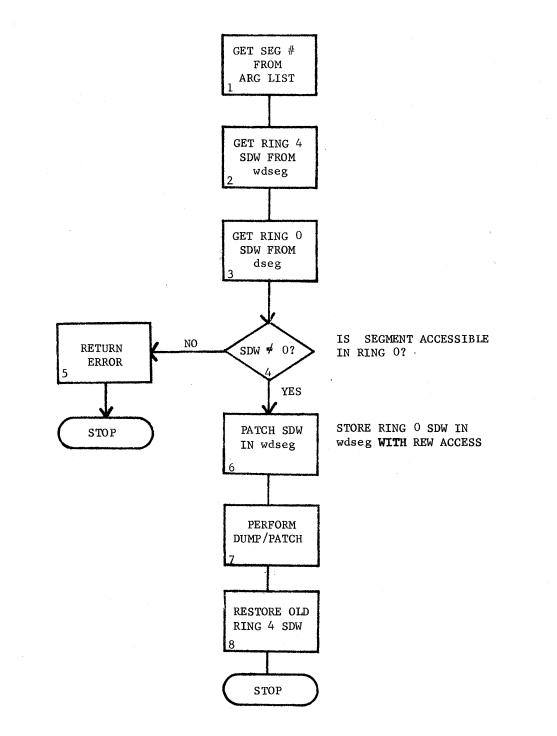
\includegraphics[scale=0.4]{images/dumpPatch.png}
    \caption{Dump/patch utility using insufficient argument validation}
    \label{dump/patch}
\end{figure}

\subsection{Violating The User Identification}

In the need for a protected identification of every user, his ID must be compared with access control list entries 
to determine whether a user may access some segment as stated in Security Controls section.
This identification is established when the user logs into Multics and is authenticated by the password.

The user identification in Multics is stored in a per-process segment called the \textit{process data segment} (PDS).
PDS resides in ring 0 and contains many constants used in ring 0 and the ring 0 procedure stack. The PDS must be 
accessible to any ring 0 procedure within a user's process and must be accessible to ring 4 master master mode 
procedures such as signaller.

Therefore as stated above section about Dump and Patch utilities vulnerability, these can dump and patch portions of the 
PDS, thus \textit{forging the non-forgeable user identification}.
This capability provides the penetrator with an ultimate exploitation weapon. The penetrator can undetechably act as any 
user of the system, including the \textit{system administrator} or \textit{security officer}, immediately assuming that 
user's access privileges.

\subsection{Value of the Password File}

The password file is often kept enciphered. A great deal of effort may be required to invert such a cipher, if the cipher 
is even invertible at all.
The password file is generally the most protected file in a computer system. If the penetrator has succeeded in breaking 
down internal controls to access the password file, he can also \textbf{access every other file in the system}.
The login path to a system is generally the most carefully audited to attempt to catch \textit{unauthorized} password use.
The penetrator risks \textit{detection} if he uses an unauthorized password.

So in this point we can assume that accessing the system password file is of minimal value to a penetrator for reasons 
stated above.

\subsection{Modifying Audit Trials}

Audit trails are frequently put into computer systems for the purpose of detecting breaches  of  security. 
For example, a record of last login time printed when a user logged in could detect the unauthorized 
use of a user’s password and identification.
Sometimes it is not convenient for the penetrator to bypass an audit, if the audit trial is kept online, 
it may be easier to allow the audit to take place and then go back and modify the evidence of wrong doing.
Every segment in Multics carries with it audit information on the \textit{Date Time last Used} (DTU) and
\textit{Date Time last Modified} (DTM). These dates are maintained by an \textit{audit mechanism} at a low 
level in the system.

A routine called "set\textunderscore dates" is provided among the various subroutine calls into ring 0, which is used when 
a segment is retrieved from a \textit{backup tape} to set the segments DTU and DTM to the values at the time the 
segment was backed up. This routine is supposed to be callable only by system maintenance personnel (ring 0).
However, since the penetrator can change his user identification, this restriction proves to be no barrier.

To access a segment penetrator simply:
\begin{enumerate}
    \item Change user ID to access segment.
    \item Remember old DTU and DTM.
    \item Use or modify the segment.
    \item Change user ID to system maintenance.
    \item --do whatever you want--
    \item Reset DTU and DTM to old values.
    \item Change user ID back to old value.
\end{enumerate}


\subsection{Trap Door Insertion}

In short, trap door is a a feature or defect of a computer system which allows surreptitious unauthorized 
access to data and system itself. When trap door is inserted, it must be well hidden to avoid detection by system
maintenance personnel.
Trap doors can be inserted in many places:
\begin{itemize}
    \item At the facility which the system is produced.
    \item During the distribution phase. If updates are sent via insecure communications.
    \item During the installation and operation of the system at user's site.
\end{itemize}

Trap doors can be easily hidden in changes to the binary code of compiled routine. Such a change can be 
detected only by comparing bit by bit the object code and the compiler listing. Which can be easily secured 
by regularly recompile of all modules of the system to eliminate such a trap doors.
However, if the compiler trap door is inserted to permit object code trap doors to survive even a complete 
recompilation of entire system. 
In Multics most of the ring 0 supervisor is written in PL/I. Penetrator could insert trap door in the PL/I and 
easily delist the desired code to be recompiled.
Since the PL/I compiler is itself written in PL/I, the trap door can \textit{maintain itself, even if the 
compiler is recompiled}.

The actual insertion of the trap door was done by following steps:
\begin{enumerate}
    \item Change user ID to project SysLib.
    \item Make patch in the object archive copy of "check\$device\underline{} name" in >ldd>hard>object.
    \item Reset DTM on object archive.
    \item Mark patch in bound archive copy of "check\$device\underline{} name" in >ldd>hard>bound\underline{}components.
    \item Reset DTM on bound archive.
    \item Reset user ID back to old value.
\end{enumerate}

\subsection{Conclusion by Schell and Karger}

The primary conclusion one can reach from this analysis is that Multics is \textit{not currently a secure system} (1973).
But on the other hand, it is \textbf{significantly more secure} than any other system.

